\chapter{Vetores}

Neste capítulo, teremos os conceitos básicos do estudo de vetores.

\section{O vetor geométrico}

Muitas quantidades físicas tais como área, comprimento, massa, temperatura, ficam completamente determinadas quando é fornecida sua magnitude (seu ``tamanho'', ``valor''). Essas quantidades são chamadas \textbf{escalares}.

Outras, no entanto, não estarão bem determinadas se, além da magnitude não são apresentados uma direção e um sentido. Essas grandezas são chamadas \textbf{vetoriais}. São exemplos de grandezas vetoriais: o movimento do vento, a força e o deslocamento.

Para compreender o conceito de vetor, as ideias de direção e sentido são fundamentais. Portanto, vamos discuti-las mais detalhadamente.

\textbf{Direção:} é aquilo que existe em comum num feixe de retas paralelas.

\textbf{Sentido:} podemos percorrer uma direção em dois sentidos.

\begin{figure}[H]
\begin{minipage}[b]{0.37\linewidth}
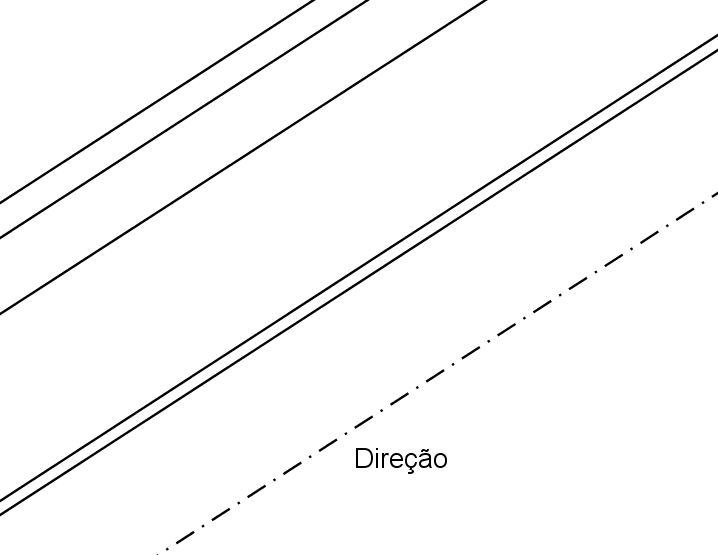
\includegraphics[width=\linewidth]{analitica/imagens/vetor1.png}
\caption{Direção}
\label{fig:direcao}
\end{minipage} \hfill
\begin{minipage}[b]{0.37\linewidth}
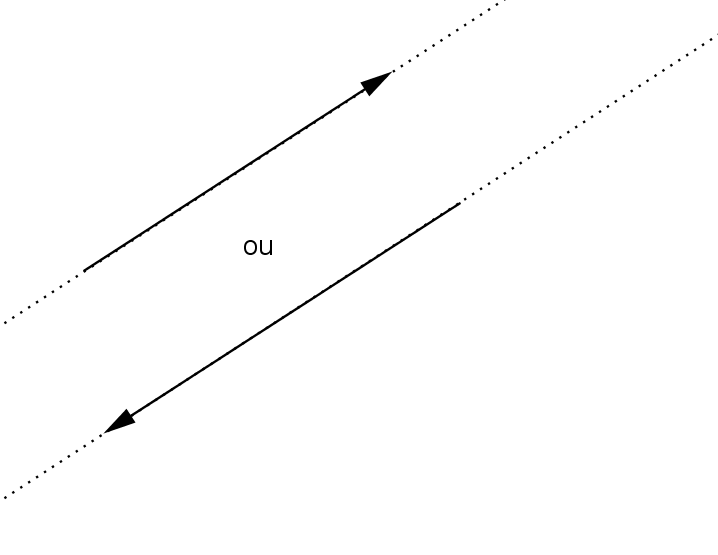
\includegraphics[width=\linewidth]{analitica/imagens/vetor2.png}
\caption{Sentido}
\label{fig:direc}
\end{minipage}
\end{figure}

Chamamos de \textbf{vetor} uma coleção de setas (ou flechas) que têm mesmo \textbf{comprimento} ou módulo, mesma \textbf{direção} e mesmo \textbf{sentido}. Cada seta é um representante do vetor. Assim, a ideia de vetor nos conduz a algo do tipo:

\begin{figure}[H]
\centering
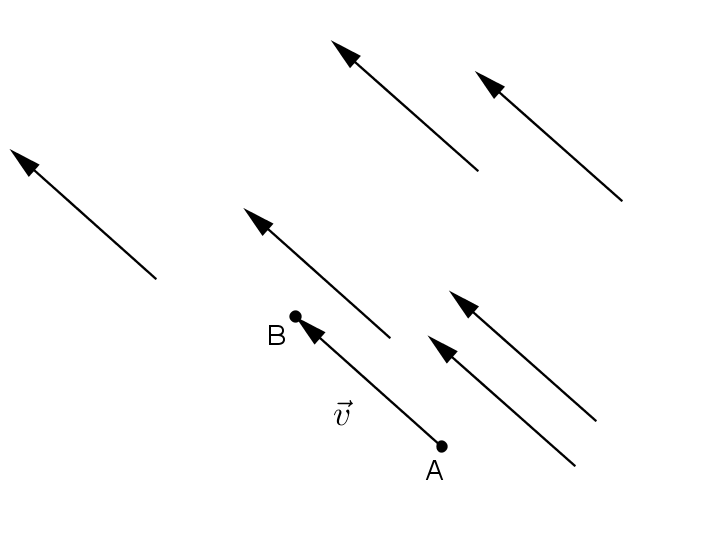
\includegraphics[scale=0.92]{analitica/imagens/vetor3.png}
\caption{Diversos representantes do mesmo vetor $\vec{v}$.}
\label{fig:vetor}
\end{figure}

\vspace{-0.4cm}
Quando escrevermos $\vec{v}=\overrightarrow{AB}$ significa que $\vec{v}$ é representado pela seta $\overrightarrow{AB}$. Porém, qualquer outra seta com o mesmo módulo (o módulo de $\vec v$ é indicado por $\Vert \vec v \Vert$), direção e sentido, representa também o mesmo vetor $\vec{v}$.

Dados os vetores $\vec{v}$ e $\vec{w}$ temos que:
\begin{enumerate}[i)]
\item o vetor de comprimento zero é chamado vetor nulo e denotado com $\overrightarrow{0}$;
\item o vetor $-\vec{v}$ é um vetor com o mesmo ``tamanho'' e mesma direção de $\vec{v}$ apenas com sentido oposto;
\item a soma dos vetores é obtida colocando a origem de $\vec{w}$ na extremidade de $\vec{v}$. O vetor soma tem origem no ponto inicial de $\vec{v}$ e extremidade no ponto final de $\vec{w}$;
 
\begin{figure}[H]
\centering
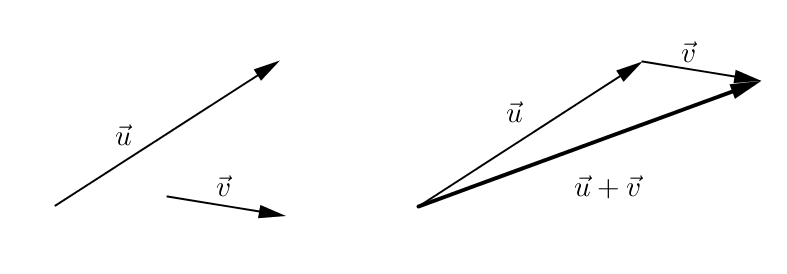
\includegraphics[scale=1.2]{analitica/imagens/vetor4.png}
\caption{Soma de dois vetores.}
\label{fig:somavetor}
\end{figure}

\vspace{-0.4cm}
\item se $k\in \mathbb{R}^{*}$ e $\vec{v}$ não é o vetor nulo, então $k\vec{v}$ é um vetor com a mesma direção de $\vec{v}$, comprimento igual a $|k|$ vezes o de $\vec{v}$, e sentido igual ao de $\vec{v}$ para $k>0$ e contrário ao de $\vec{v}$ para $k<0$.
\end{enumerate}

\subsection{Casos particulares de vetores}

Para a continuação do estudo, é preciso que identifiquemos situações específicas de vetores:
\begin{enumerate}[(1)]
 \item \textbf{paralelos} - Dois vetores $\vec u$ e $\vec v$ são \textit{paralelos}, e indica-se por $\vec u \parallel \vec v$, se os seus representantes tiverem a mesma direção.
 \item \textbf{iguais} - Dois vetores $\vec u$ e $\vec v$ são \textit{iguais}, e indica-se por $\vec u=\vec v$, se tiverem o mesmo módulo, mesma direção e mesmo sentido.
 \item \textbf{unitário} - É chamado de vetor \textit{unitário} aquele que tiver comprimento ou módulo igual a 1. Se $\Vert \vec v \Vert\neq 0$, o \textit{versor} de $\vec v$ é o vetor unitário com mesma direção e sentido de $\vec v$. Por exemplo, se $\Vert \vec v \Vert =3$, então o versor de $\vec v$ será $\frac{\vec v}{\Vert \vec v \Vert}=\frac{\vec v}{3}$.
 \item \textbf{oposto} - A cada vetor não-nulo $\vec v$ é associado um vetor \textit{oposto} $-\vec v$, que possui mesmo módulo e direção, mas sentido contrário de $\vec v$.
 \item \textbf{ortogonais} - Dois vetores $\vec u$ e $\vec v$ são \textit{ortogonais}, indicando-se $\vec u \perp \vec v$, se algum representante de $\vec u$ formar ângulo reto com algum representante de $\vec v$.
 \item \textbf{coplanares} - Dois ou mais vetores são \textit{coplanares} se existir algum plano onde estes vetores estão representados. Observe que \textit{dois vetores} são sempre coplanares, pois basta escolher um ponto $P$ e representar ambos a partir deste ponto. 
\end{enumerate}

\section{Abordagem algébrica: vetores no plano}

\begin{df}
Um vetor $\vec{v}$ é representado por diferentes setas no plano cartesiano.
\end{df}

\begin{figure}[H]
\centering
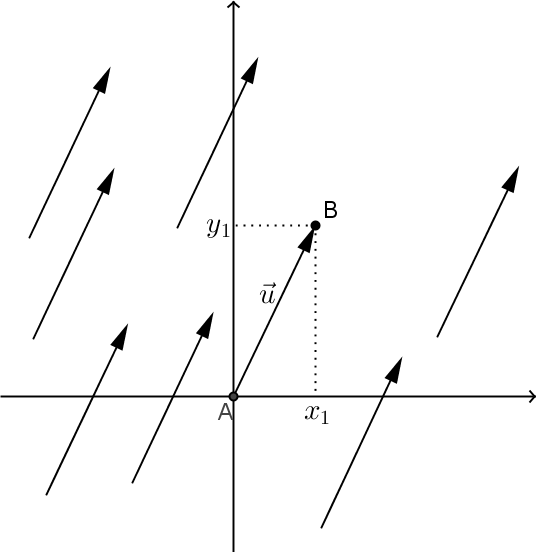
\includegraphics[scale=1.2]{analitica/imagens/vetor5.png}
\caption{Vetores no plano.}
\label{fig:vetorplano}
\end{figure}

Posicionando $\vec{v}$ com seu ponto inicial na origem do sistema, as coordenadas do ponto $B(x_1, y_1)$ (seu ponto final) são chamadas de componentes de $\vec{v}$ e escrevemos $\vec{v}=(x_1, y_1)$. A seta $\overrightarrow{AB}$ é chamada de representação posicional de $\vec{v}$.

\begin{exemplo} trace a representação posicional de $\vec{v}=(4, 2)$ e responda qual o:

\begin{figure}[H]
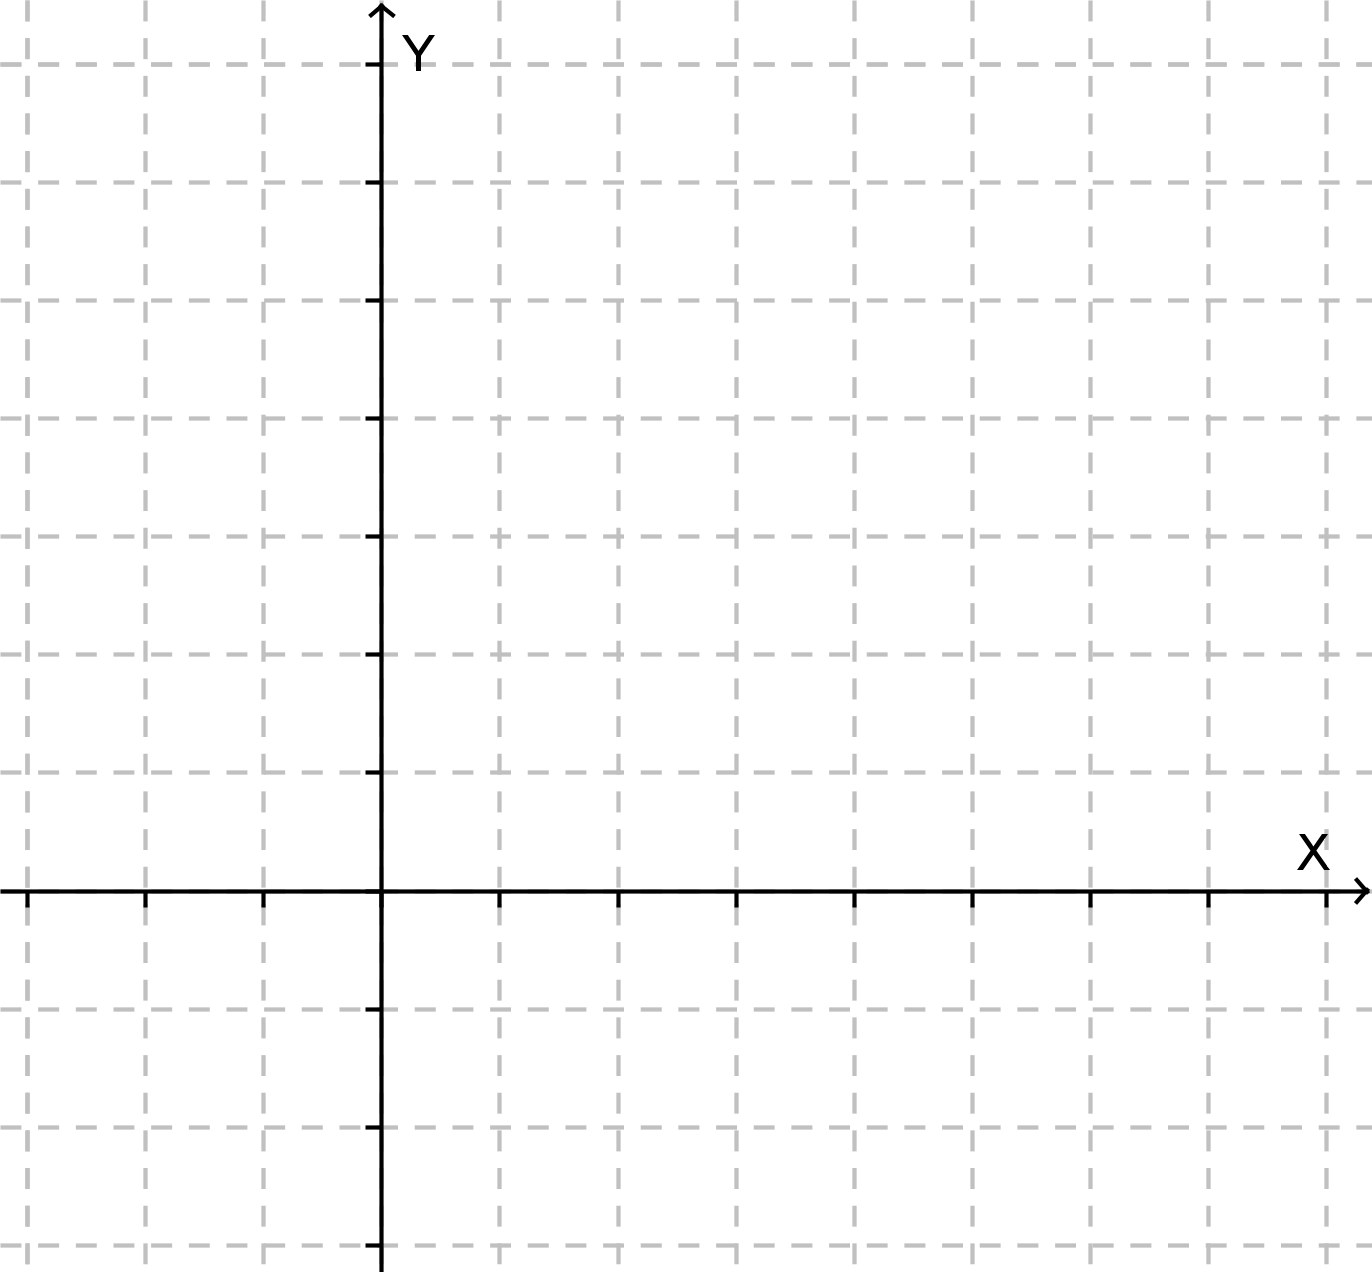
\includegraphics[scale=0.47]{analitica/imagens/malha.png}
\end{figure}

\begin{enumerate}[a)]
  \item ponto terminal de $\vec{v}$, se o ponto inicial for $(-2, 3)$.
  \item ponto inicial de $\vec{v}$, se o ponto terminal for $(6, 1)$.
\end{enumerate}
\end{exemplo}

\begin{df}
Os vetores $\vec{u}=(x_1, y_1)$ e $\vec{v}=(x_2, y_2)$ são iguais se e somente se $x_1=x_2$ e $y_1=y_2$.
\end{df}

\subsection{Operações com vetores}

Dados os vetores $\vec{u}=(x_1, y_1)$ e $\vec{v}=(x_2, y_2)$ temos que:

\begin{itemize}
\item $\vec{u}+\vec{v}=(x_1+x_2, y_1+y_2)$
\item $\vec{u}-\vec{v}=(x_1-x_2, y_1-y_2)$
\item $k\cdot \vec{u}=(k\cdot x_1, k\cdot y_1)$
\end{itemize}

\begin{exemplo} Sendo $\vec{u}=(3, 1)$ e $\vec{v}=(1, 2)$, determine o que é pedido:

\begin{figure}[H]
\begin{minipage}[b]{0.3\linewidth}
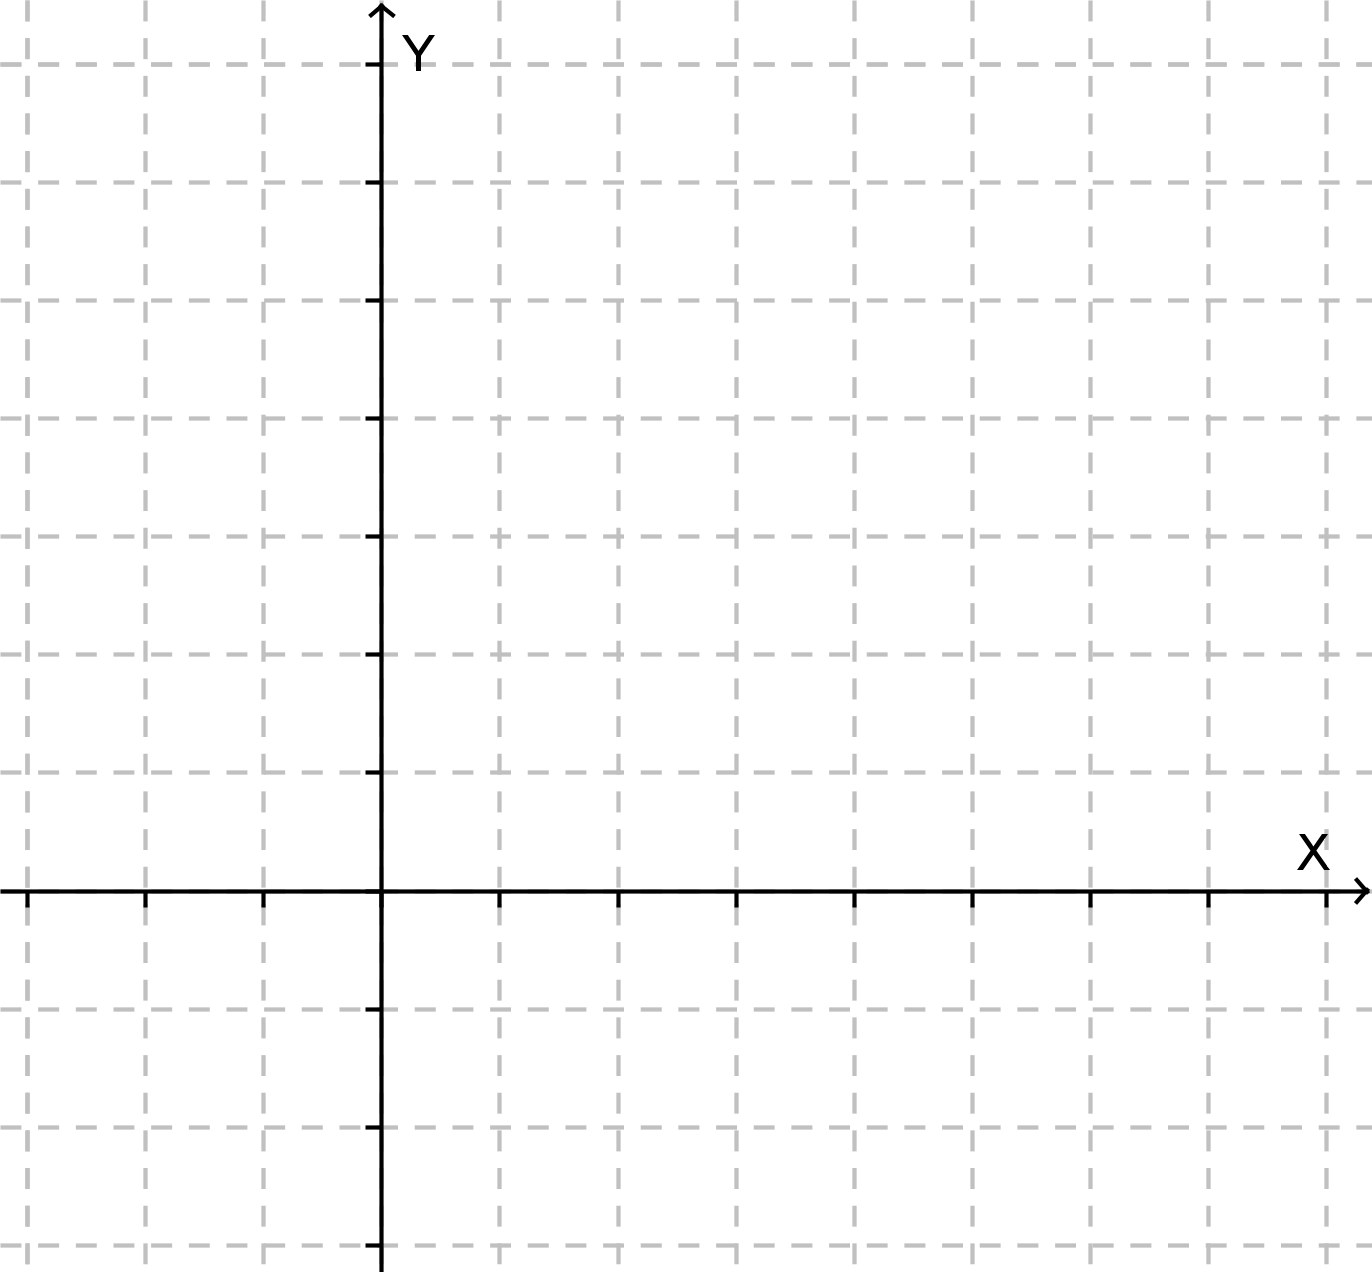
\includegraphics[width=\linewidth]{analitica/imagens/malha.png}
\caption{a) $\vec{u}+\vec{v}=$}
\end{minipage} \hfill
\begin{minipage}[b]{0.3\linewidth}
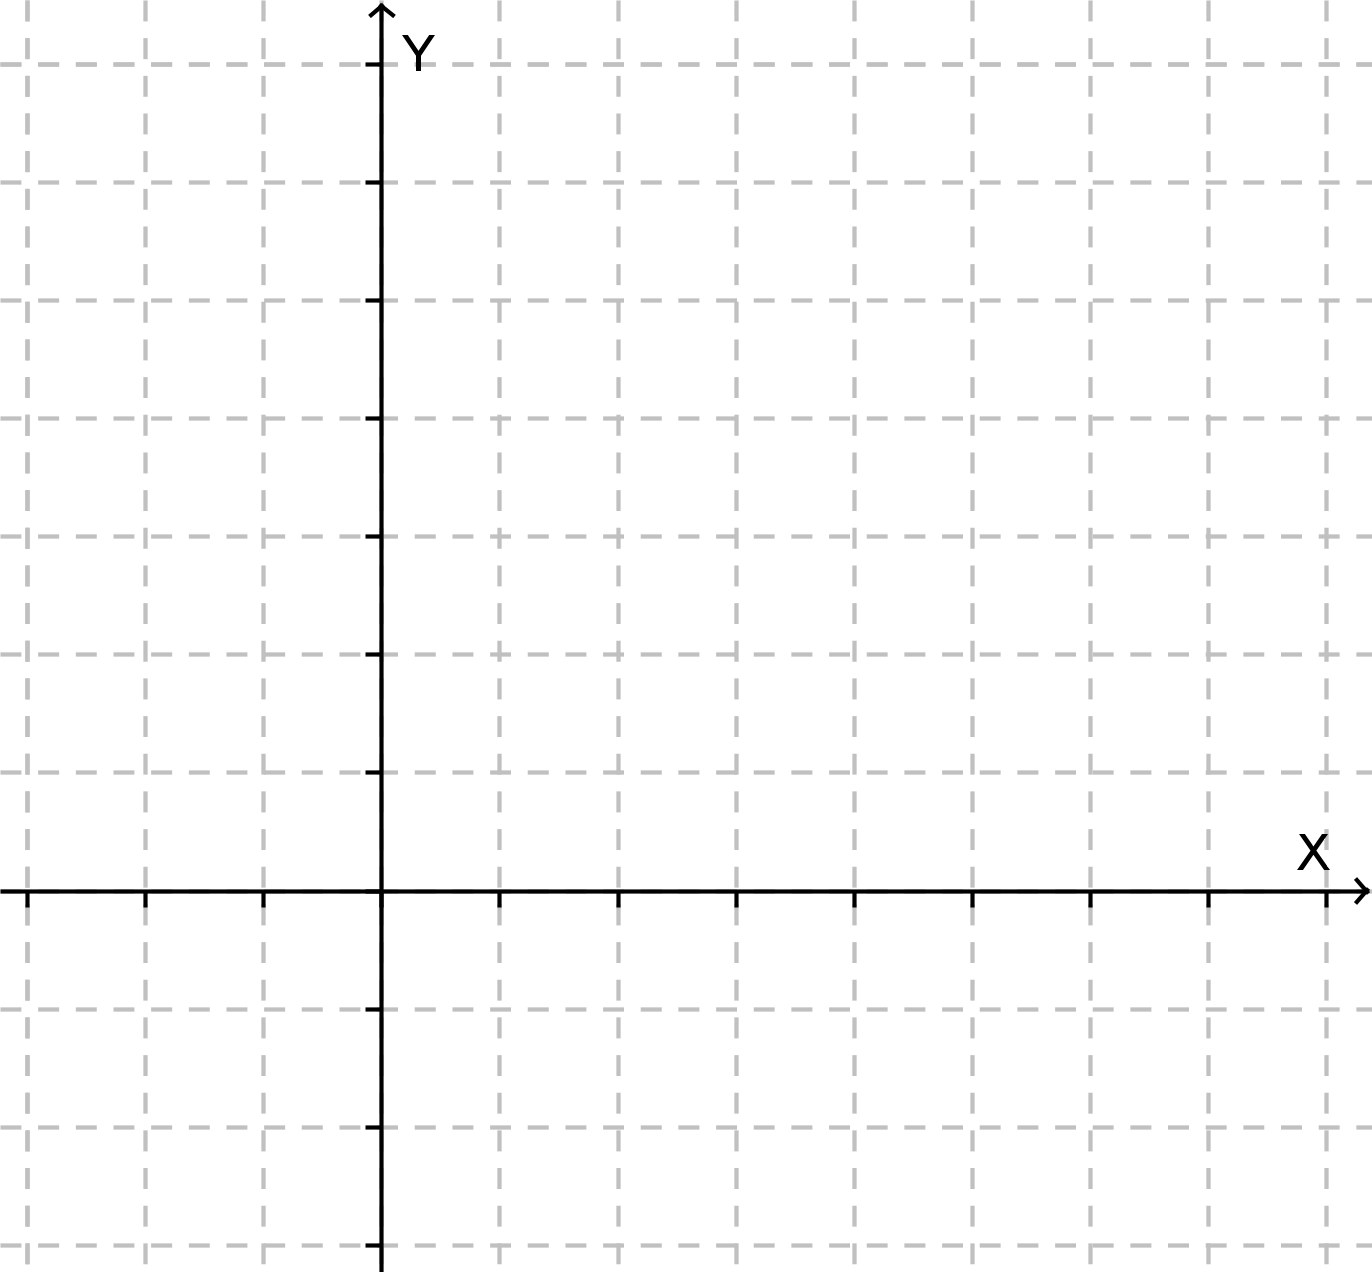
\includegraphics[width=\linewidth]{analitica/imagens/malha.png}
\caption{b) $\vec{u}-\vec{v}=$}
\end{minipage}\hfill
\begin{minipage}[b]{0.3\linewidth}
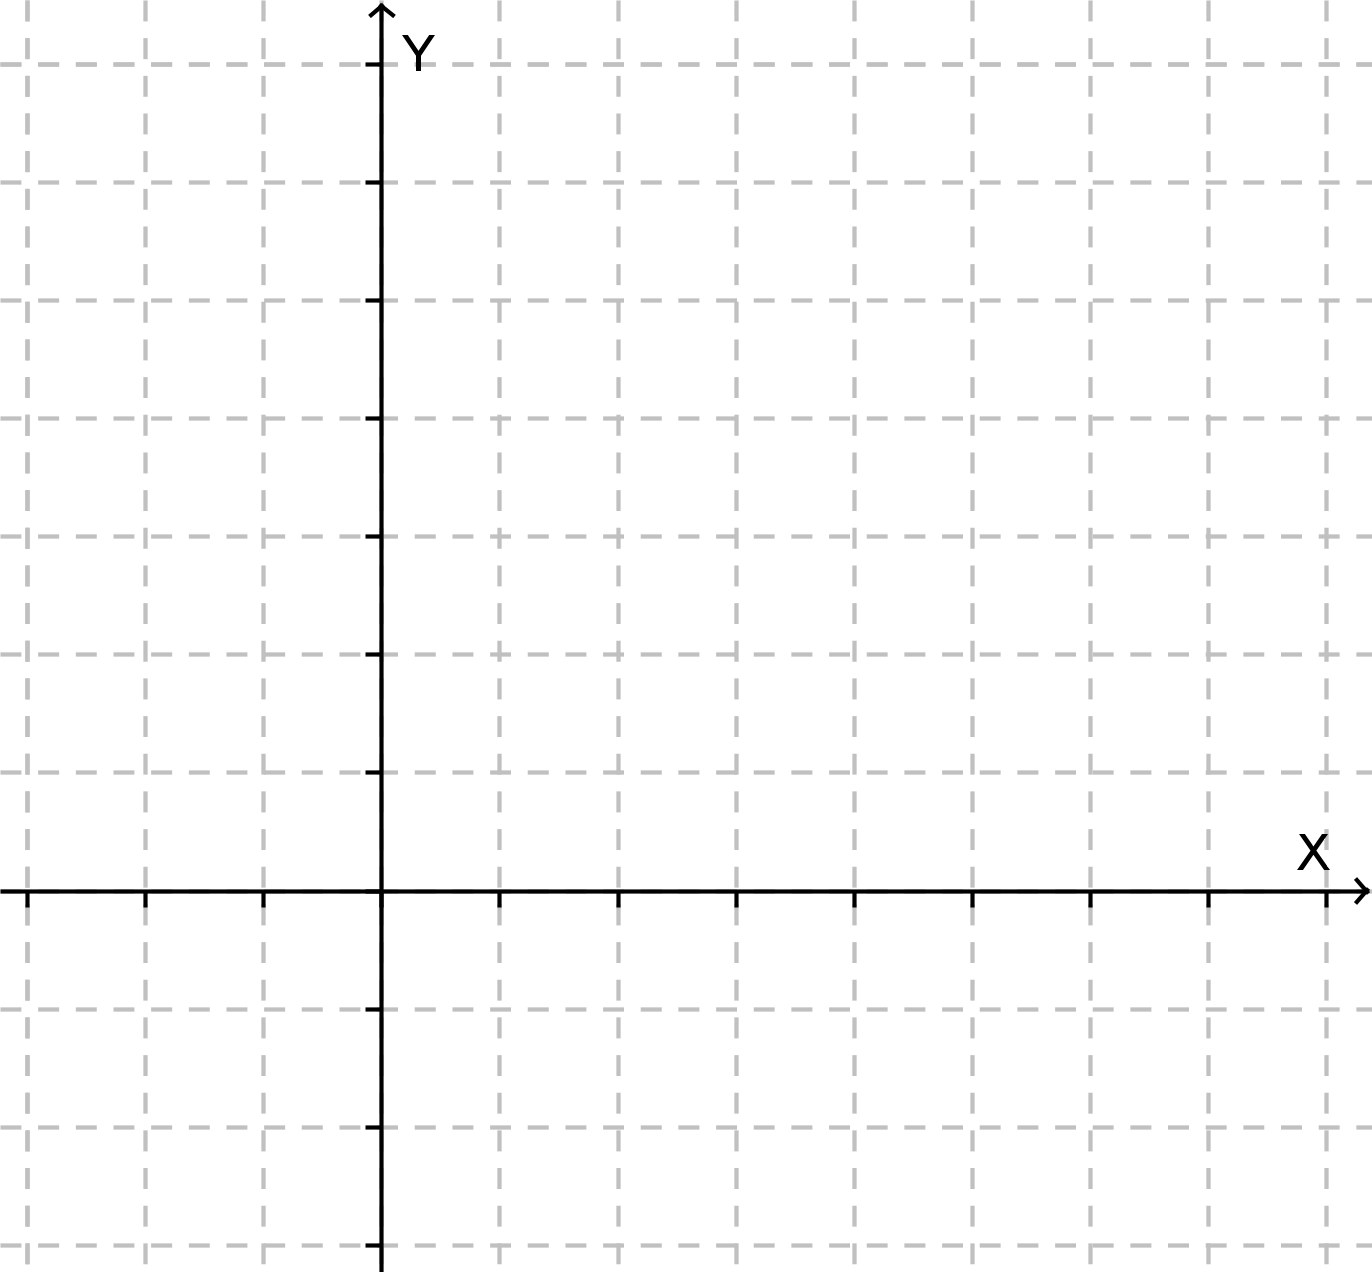
\includegraphics[width=\linewidth]{analitica/imagens/malha.png}
\caption{c) $3\cdot \vec{v}=$}
\end{minipage}
\end{figure}

d) $a$ e $b$ sabendo que $a\cdot \vec{u}+b\cdot \vec{v}=(9, 8)$.
\end{exemplo}
\vspace{2cm}

\subsection{Expressão analítica de um vetor}

Consideremos agora o vetor $\vec{i}=(1,0)$ e $\vec{j}=(0,1)$. Será que poderemos dizer que o vetor $\vec{v}=(2,3)$, por exemplo, pode ser escrito como $\vec{v}=2\vec{i}+3\vec{j}$? Verifique graficamente.

É fácil ver que esse fato ocorre para todo vetor do plano. Mais tarde estudaremos que esses vetores $\vec{i}$ e $\vec{j}$ formam uma base do $\mathbb{R}^2$. Isto é, dado um vetor $\vec{v}$, existe um único par de números reais, $x$ e $y$, tais que $\vec{v}=x\vec{i}+y\vec{j}$.

\begin{figure}[H]
\centering
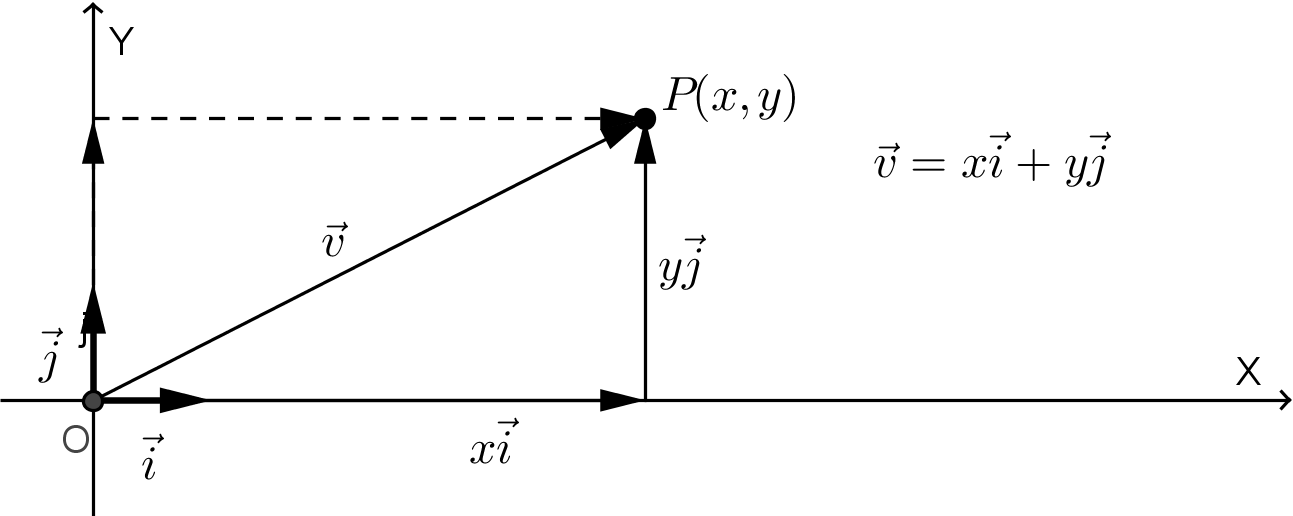
\includegraphics[scale=0.82]{analitica/imagens/combinalinear.png}
\end{figure}

\subsection{Vetor definido por dois pontos}

Muitas vezes um vetor é representado por uma seta que não parte da origem do sistema. Sendo $\vec{v}=\overrightarrow{AB}$, com $A(x_a, y_a)$ e $B(x_b, y_b)$, como podemos determinar as componentes de $\vec{v}$?

\begin{multicols}{2}
\begin{figure}[H]
\centering
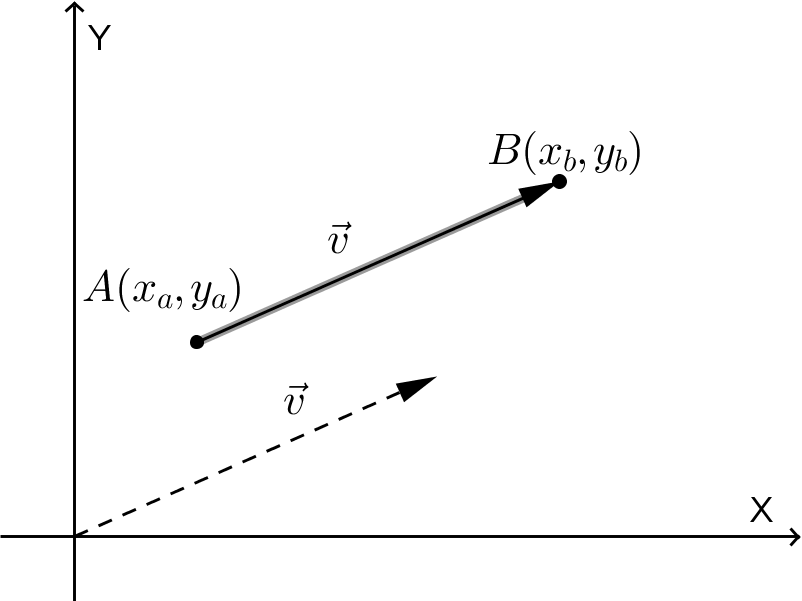
\includegraphics[scale=0.87]{analitica/imagens/doispontos.png}
\end{figure}

$$\vec{v}=\overrightarrow{AB}=\ldots$$
\end{multicols}


\begin{exemplo} sendo $A(1, 2)$, $B(7, 3)$ e $C(5, 7)$, determine os vetores:
\begin{enumerate}[a)]
 \item $\overrightarrow{AB}$
 \item $\overrightarrow{CB}$
 \item $\overrightarrow{AC}$
\end{enumerate}
\end{exemplo}

\subsection{Paralelismo de vetores}

Se dois vetores $\vec{u}$ e $\vec{v}$ são paralelos, então existe um número $\alpha$ tal que $\vec{u}=\alpha \vec{v}$.

Se $\vec{u}=(x_1, y_1)$ e $\vec{v}=(x_2, y_2)$ então $(x_1, y_1)=\alpha(x_2, y_2)$ e portanto $x_1=\alpha x_2$ e $y_1=\alpha y_2$ de onde se conclui que $\displaystyle \alpha=\frac{x_1}{x_2}=\frac{y_1}{y_2}$. Logo

$$\vec{u} \parallel \vec{v}  \qquad \Longleftrightarrow \qquad \frac{x_1}{x_2}=\frac{y_1}{y_2}$$

Observações:
\begin{enumerate}[a)]
 \item o vetor nulo $\vec{0}=(0, 0)$ é paralelo a qualquer vetor.
 \item se uma das componentes do vetor $\vec{v}$ é nula, a componente correspondente de qualquer vetor paralelo a $\vec{v}$ também é nula.
\end{enumerate}

\subsection{Módulo ou norma de um vetor}

A distância entre os pontos inicial e final do segmento orientado que representa um vetor $\vec{v}$ é chamada de módulo de \textit{módulo} ou \textit{norma} de $\vec{v}$ e denotada por $\Vert\vec{v}\Vert$. 

Essa distância não muda se o vetor for transladado, logo, para propósitos  de  cálculo  da  norma, podemos supor que o vetor está posicionado com seu ponto inicial na origem.

\begin{figure}[H]
\centering
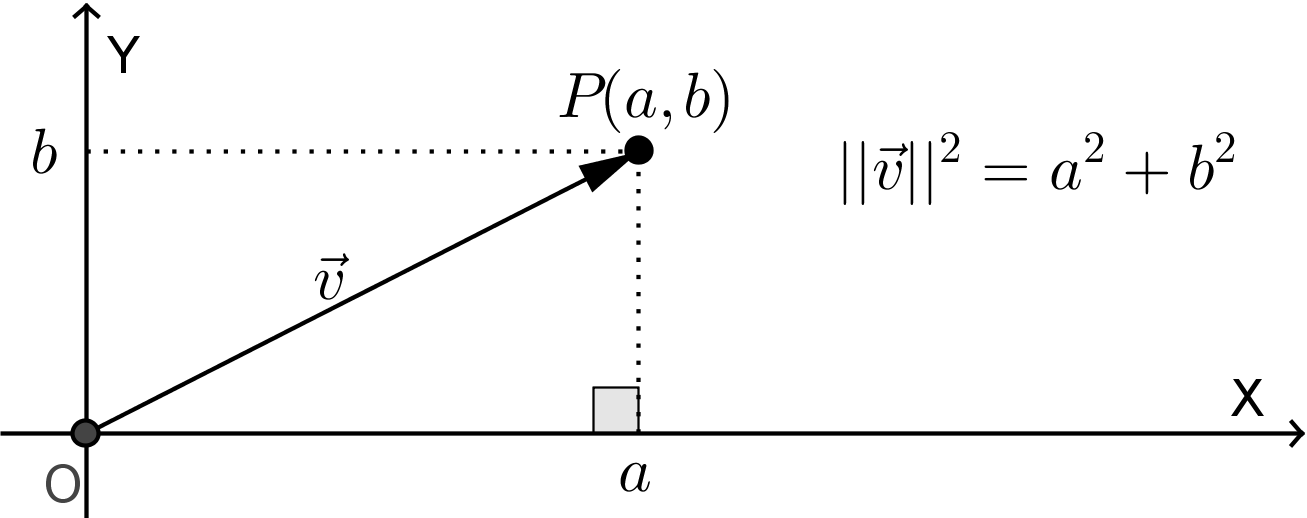
\includegraphics[scale=0.8]{analitica/imagens/norma.png}
\end{figure}

Pelo teorema de Pitágoras temos que a norma do vetor $\vec{v}=(a)$ é dada por: $$\Vert\vec{v}\Vert=\sqrt{a^2+b^2}$$

\begin{exemplo} sendo $\vec{v}=(4, 2)$, determine:

\begin{enumerate}[a)]
 \item o módulo de $\vec{v}$. \vspace{1cm}
 \item um vetor unitário com mesma direção e sentido de $\vec{v}$. \vspace{1cm}
 \item um vetor unitário com mesma direção e sentido contrário de $\vec{v}$. \vspace{2cm}
\end{enumerate}
\end{exemplo}

\section{Abordagem algébrica: vetores no espaço}

Como os elementos do $\mathbb{R}^2$ e $\mathbb{R}^3$ são representados, respectivamente, por pares $(x,y)$ e ternas $(x,y,z)$, estes elementos podem ser interpretados como pontos ou vetores. Então, $(x,y)$ e $(x,y,z)$ são as coordenadas de um ponto que marca uma posição ou de um vetor que define um deslocamento.

No espaço, como todo elemento do $\mathbb{R}^3$, os vetores serão representados por três componentes: $$\vec v=(a,b,c)$$

\begin{figure}[H]
\centering
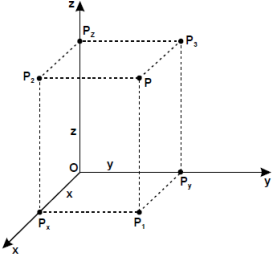
\includegraphics[scale=0.7]{analitica/imagens/vetor-r3-3.png}
\end{figure}

No plano, os vetores $\vec i=(1,0)$ e $\vec j=(0,1)$ formam uma base do $\mathbb{R}^2$, e com isso um vetor $\vec v=(a,b)$ pode ser escrito como $\vec v=a\vec i+b\vec j$.

No espaço, os vetores $\vec i=(1,0,0)$, $\vec j=(0,1,0)$ e $\vec k=(0,0,1)$ formam uma base do $\mathbb{R}^3$, e com isso um vetor $\vec v=(a,b,c)$ pode ser escrito como $\vec v=a\vec i+b\vec j+c\vec k$.

As relações algébricas para o espaço, são análogas ao do plano, pois basta acrescentar uma componente na representação:
\begin{enumerate}[I)]
 \item Dois vetores $\vec u=(x_1, y_1, z_1)$ e $\vec v=(x_2, y_2, z_2)$ são \textbf{iguais} se, e somente se, $x_1=x_2$, $y_1=y_2$ e $z_1=z_2$.
 \item Dados os vetores $\vec u=(x_1, y_1, z_1)$ e $\vec v=(x_2, y_2, z_2)$ e $\alpha \in \mathbb{R}^2$, define-se:
   \begin{enumerate}
     \item $\vec u +\vec v=(x_1+x_2, y_1+y_2, z_1+z_2)$
     \item $\alpha \vec u=(\alpha x_1, \alpha y_1, \alpha z_1)$
   \end{enumerate}
 \item Se $A=(x_1, y_1, z_1)$ e $B=(x_2, y_2, z_2)$ são \textbf{dois pontos} quaisquer do espaço, então $\overrightarrow{AB}=B-A=(x_2-x_1, y_2-y_1, z_2-z_1)$. E se $\vec v=\overrightarrow{AB}=B-A$, então $$B=A+\vec v$$
 \item Se os vetores $\vec u=(x_1, y_1, z_1)$ e $\vec v=(x_2, y_2, z_2)$ são \textbf{paralelos}, então $\vec u=\alpha \vec v$ ou $$\frac{x_1}{x_2}=\frac{y_1}{y_2}=\frac{z_1}{z_2}$$

Observações:
 \begin{enumerate}[a)]
  \item o vetor nulo $\vec{0}=(0, 0, 0)$ é paralelo a qualquer vetor.
  \item se uma das componentes do vetor $\vec{v}$ é nula, a componente correspondente de qualquer vetor paralelo a $\vec{v}$ também é nula.
 \end{enumerate}
 
 \item O \textbf{comprimento} (norma ou módulo) do vetor $\vec v=(a, b, c)$ é dado por $$\Vert \vec v \Vert=\sqrt{a^2+b^2+c^2}$$

\end{enumerate}

\section{Combinação linear de vetores}

Sejam os vetores $\vec v_1, \vec v_2, \vec v_3, \ldots, \vec v_n $. Um vetor $v$ é combinação linear (CL) dos vetores $\vec v_1, \vec v_2, \vec v_3, \ldots, \vec v_n $ se existirem as constantes $a_1, a_2, a_3, \ldots, a_n \in \mathbb{R}$, tais que $$\vec v=a_1\vec v_1+a_2\vec v_2+a_3\vec v_3+\ldots+a_n\vec v_n$$

Nem sempre é possível expressar um dado vetor como combinação linear de outros dois e, quando possível, pode existir mais de uma solução. Para entender esta afirmação, repare que este problema é equivalente a achar a solução de um sistema de equações lineares. O número de componentes do vetor fornece o número de equações do sistema. Se o sistema for determinado será possível resolver o problema dado.